\documentclass{article}
\usepackage[utf8]{inputenc}
\usepackage{enumitem}
\usepackage{bm}
\usepackage[margin=1.0in]{geometry}

\title{Physics 116B \\ Mathematical Methods in Physics\\ Small Group Tutoring}
\author{Pablo Sevilla}
\date{Week 2}

\usepackage{natbib}
\usepackage{graphicx}

\begin{document}
\maketitle

\begin{figure}[h]
\centering

\includegraphics[scale=0.3]{lss}
\end{figure}
\section{Preliminary Questions}
 \begin{itemize}
  \item Explain qualitatively how the following matrix equation relates to transformations.
  \begin{figure}[h]
\centering
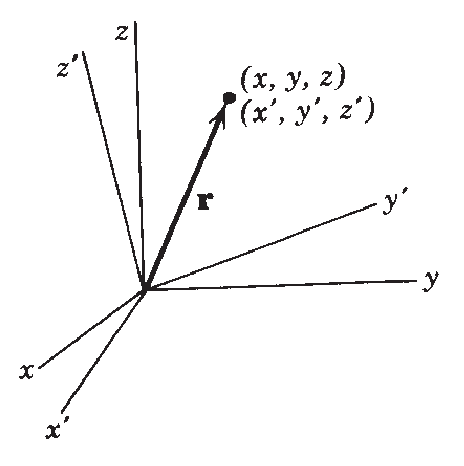
\includegraphics[scale=0.2]{1}
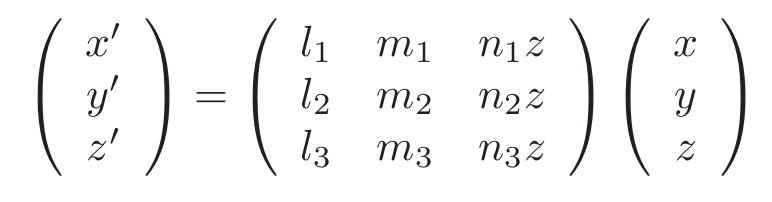
\includegraphics[scale=0.3]{2}
\end{figure}
\item Write out each summation:
\begin{equation}
    \sum_{i=1}^{3} a_{ii}
\end{equation}
\begin{equation}
    \sum_{i=1}^{5} x_{i}x_i
\end{equation}
\begin{equation}
    \sum_{j=1}^{3} \sum_{i=1}^{3} u_{ij}v_{ji}
\end{equation}
  \item For a rotating rigid body, the torque is calculated using $\bm{\tau}=\frac{d\bm{L}}{dt}$. Explain what it is meant by each term in the equation $\bm{L}=I\bm{w}$. Under what conditions are $\bm{L}$ and $\bm{w}$ parallel?
  \item Write out the mathematical definitions for the Kronocker Delta $\delta_{ii}$ and the Levi-Civita Symbol $\epsilon_{ijk}$. 
  \end{itemize}
  \clearpage
  \section{Group Problems}
  Work together as a group for the following problems. Once solved, prepare a presentation to explain the problems in an organized manner.
  \subsection{Problem 1}
  Rotations can be described by using the nine angles between the two coordinates systems, $(x, y, z)$ and $(x', y', z')$. Show that such angles in matrix form form an orthonormal set.
  
Hint: Use linear algebra properties.
  \subsection{Problem 2}
  Show that the contracted tensor $T_{ijk}V_k$ is a $2^{nd}$ rank tensor.
  $T_{ijk}$ and $V_k$ are defined as follows:
  \begin{equation}
      V_k = \sum_{i=1}^{3} a_{\tau k}V'_{\tau}}
  \end{equation}
  \begin{equation}
    T_{ijk} = \sum_{i=1}^{3} \sum_{j=1}^{3} \sum_{k=1}^{3} 
    a_{\alpha i}a_{\beta j}a_{\gamma k} T'_{\alpha \beta \gamma}
  \end{equation}
  Hint: Use that fact that $a_{ij}a_{kj}=\delta_{ik}$ and check how many free indices you have left.
  \subsection{Problem 3}
  Evaluate the following products:
  \begin{enumerate}
  \centering
      \item \delta_{ij}\delta_{jk}\delta_{km}\delta_{im}
      
      \item \epsilon_{jk2}\epsilon_{k2j}
      
      \item \epsilon_{23i}\epsilon_{2i3}
      
  \end{enumerate}
  
  Hint for 1: Set $j=1$, then $k=i$ and finally $m=i$.
  
  Hint for 2: Take advantage of the fact that $\epsilon_ijk$ is anti-symmetric and $\delta_jk$ is symmetric. Interchange k and j in the final step that allows you to evaluate.
  
  Hint for 3: The product of two permutations can be evaluated using a 3x3 matrix of the constituent Kronocker Delta functions.
  
\end{document}
